\documentclass[11pt,a3paper,landscape]{article}
\usepackage[utf8]{inputenc}
\usepackage[T1]{fontenc}
\usepackage[paperwidth=42cm,paperheight=29.7cm,margin=0.8cm]{geometry}
\usepackage{tikz}
\usepackage{graphicx}
\usetikzlibrary{arrows.meta,positioning,fit,backgrounds,calc}

\definecolor{pastelRuntime}{RGB}{220,234,252}
\definecolor{pastelApi}{RGB}{226,245,230}
\definecolor{pastelViews}{RGB}{227,242,253}
\definecolor{pastelServices}{RGB}{255,239,219}
\definecolor{pastelSchemas}{RGB}{236,230,252}
\definecolor{pastelExceptions}{RGB}{255,243,214}

\begin{document}
\pagestyle{empty}

\begin{center}
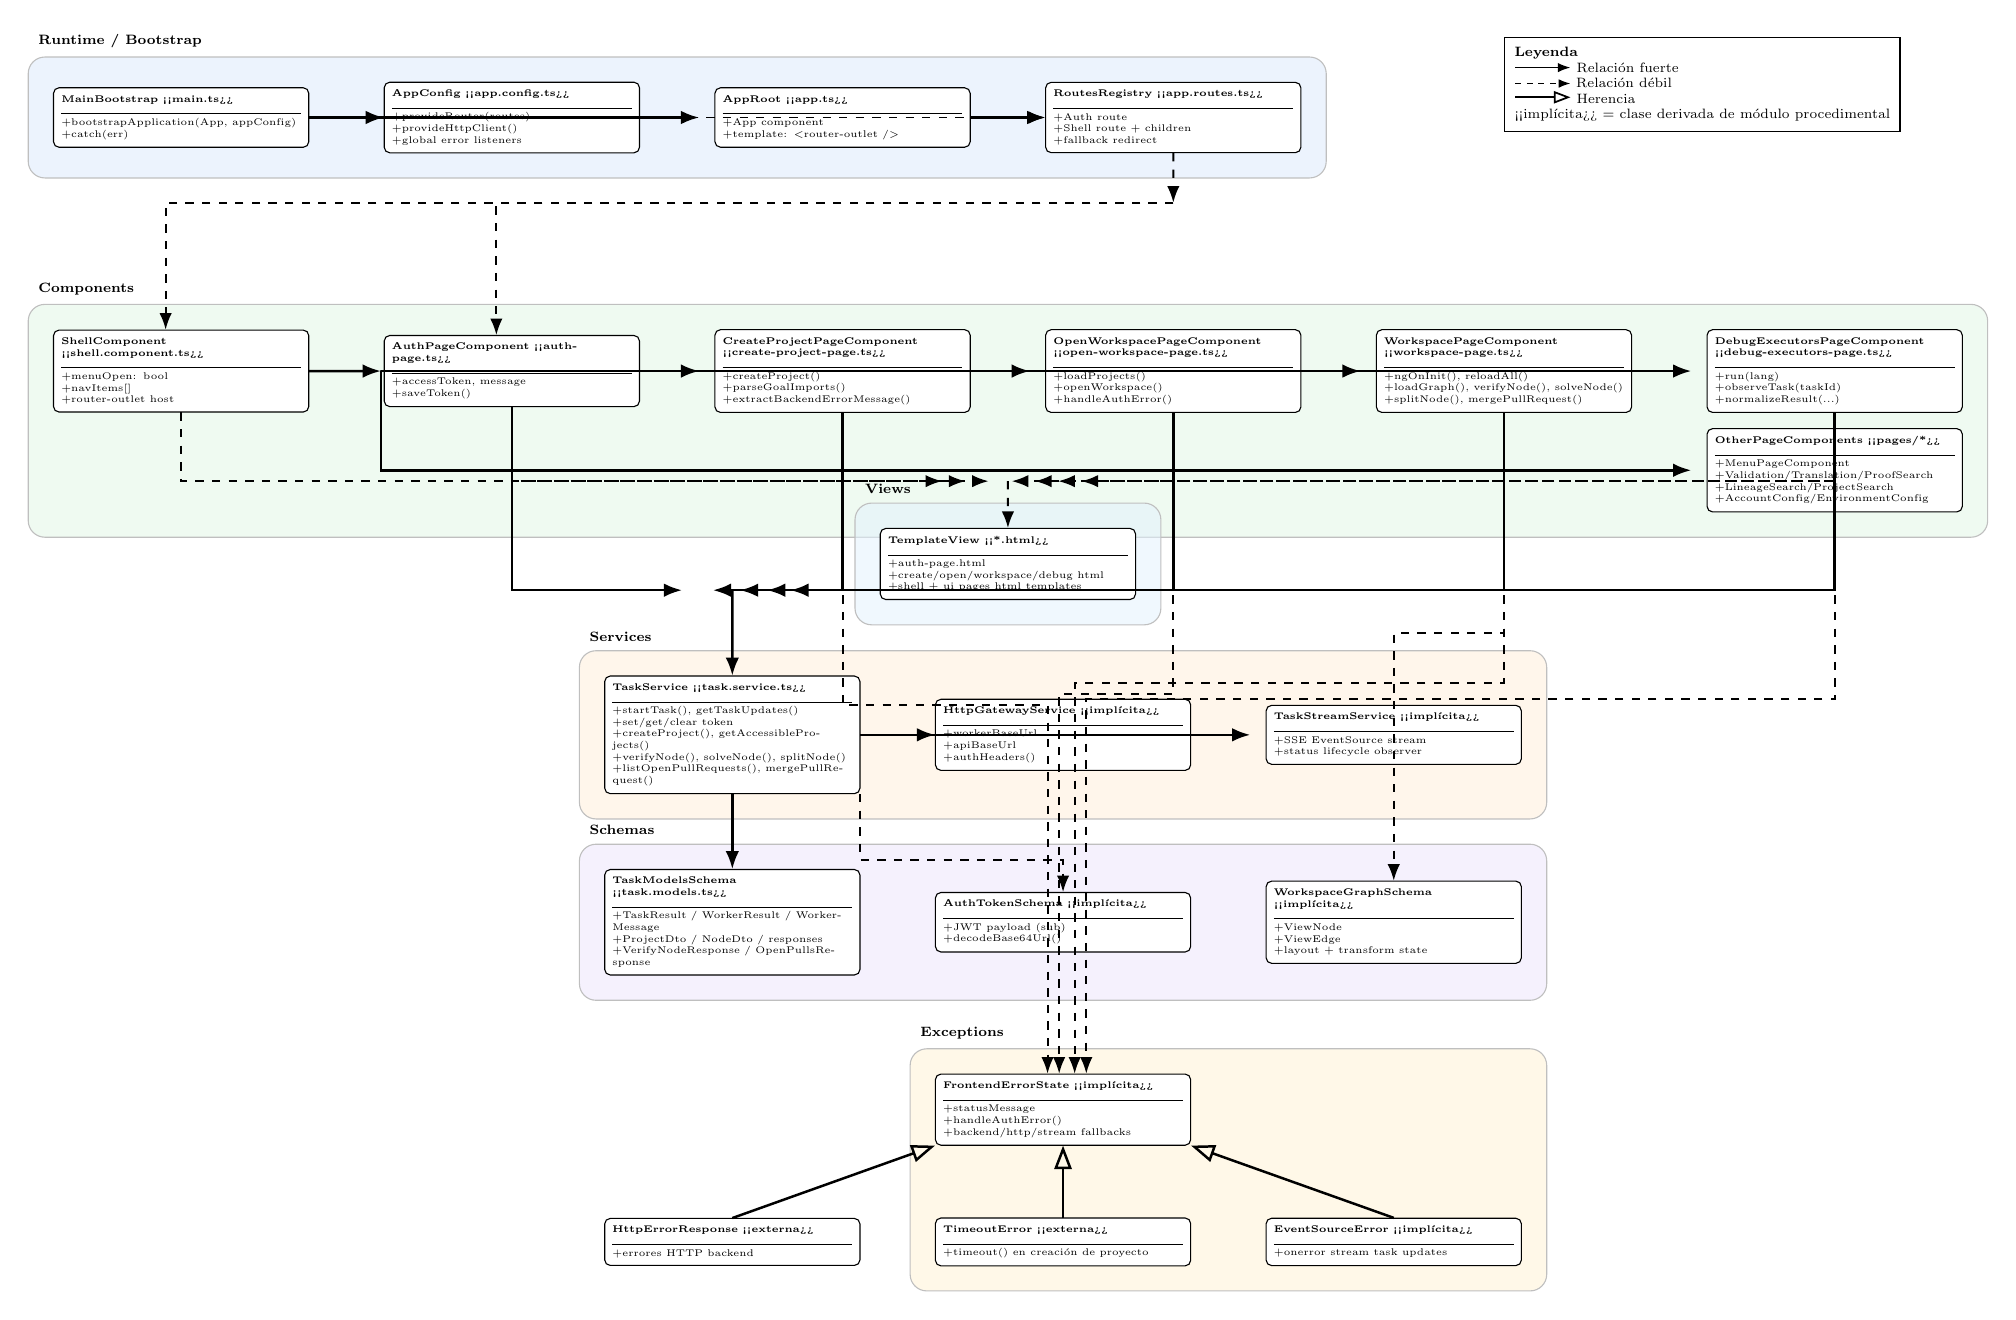
\begin{tikzpicture}[
  scale=0.70,
  transform shape,
  x=1cm,
  y=1cm,
  classbox/.style={
    draw,
    rounded corners=2pt,
    align=left,
    font=\tiny,
    text width=4.35cm,
    inner sep=4pt,
    fill=white
  },
  sectionbox/.style={draw=black!25, line width=0.4pt, rounded corners=6pt, inner sep=9pt, fill opacity=0.55},
  strong/.style={-{Latex[length=2.3mm]}, line width=0.9pt},
  weak/.style={-{Latex[length=2.1mm]}, line width=0.7pt, dashed},
  inherit/.style={-{Triangle[open,length=3mm,width=2.2mm]}, line width=0.9pt},
  rel/.style={font=\tiny, fill=white, inner sep=1pt}
]

% =========================
% Runtime / Bootstrap
% =========================
\node[classbox] (bootstrap) at (0,12.2) {
\textbf{MainBootstrap <<main.ts>>}\\
\rule{\linewidth}{0.2pt}\\
+bootstrapApplication(App, appConfig)\\
+catch(err)
};

\node[classbox] (appConfig) at (6.0,12.2) {
\textbf{AppConfig <<app.config.ts>>}\\
\rule{\linewidth}{0.2pt}\\
+provideRouter(routes)\\
+provideHttpClient()\\
+global error listeners
};

\node[classbox] (appRoot) at (12.0,12.2) {
\textbf{AppRoot <<app.ts>>}\\
\rule{\linewidth}{0.2pt}\\
+App component\\
+template: <router-outlet />
};

\node[classbox] (routesRegistry) at (18.0,12.2) {
\textbf{RoutesRegistry <<app.routes.ts>>}\\
\rule{\linewidth}{0.2pt}\\
+Auth route\\
+Shell route + children\\
+fallback redirect
};

% =========================
% Components
% =========================
\node[classbox] (shellCtrl) at (0,7.6) {
\textbf{ShellComponent <<shell.component.ts>>}\\
\rule{\linewidth}{0.2pt}\\
+menuOpen: bool\\
+navItems[]\\
+router-outlet host
};

\node[classbox] (authCtrl) at (6.0,7.6) {
\textbf{AuthPageComponent <<auth-page.ts>>}\\
\rule{\linewidth}{0.2pt}\\
+accessToken, message\\
+saveToken()
};

\node[classbox] (createProjectCtrl) at (12.0,7.6) {
\textbf{CreateProjectPageComponent <<create-project-page.ts>>}\\
\rule{\linewidth}{0.2pt}\\
+createProject()\\
+parseGoalImports()\\
+extractBackendErrorMessage()
};

\node[classbox] (openWorkspaceCtrl) at (18.0,7.6) {
\textbf{OpenWorkspacePageComponent <<open-workspace-page.ts>>}\\
\rule{\linewidth}{0.2pt}\\
+loadProjects()\\
+openWorkspace()\\
+handleAuthError()
};

\node[classbox] (workspaceCtrl) at (24.0,7.6) {
\textbf{WorkspacePageComponent <<workspace-page.ts>>}\\
\rule{\linewidth}{0.2pt}\\
+ngOnInit(), reloadAll()\\
+loadGraph(), verifyNode(), solveNode()\\
+splitNode(), mergePullRequest()
};

\node[classbox] (debugCtrl) at (30.0,7.6) {
\textbf{DebugExecutorsPageComponent <<debug-executors-page.ts>>}\\
\rule{\linewidth}{0.2pt}\\
+run(lang)\\
+observeTask(taskId)\\
+normalizeResult(...)
};

\node[classbox] (uiPagesCtrl) at (30.0,5.8) {
\textbf{OtherPageComponents <<pages/*>>}\\
\rule{\linewidth}{0.2pt}\\
+MenuPageComponent\\
+Validation/Translation/ProofSearch\\
+LineageSearch/ProjectSearch\\
+AccountConfig/EnvironmentConfig
};

% =========================
% Views
% =========================
\node[classbox] (templateView) at (15.0,4.1) {
\textbf{TemplateView <<*.html>>}\\
\rule{\linewidth}{0.2pt}\\
+auth-page.html\\
+create/open/workspace/debug html\\
+shell + ui pages html templates
};

% =========================
% Services
% =========================
\node[classbox] (taskService) at (10.0,1.0) {
\textbf{TaskService <<task.service.ts>>}\\
\rule{\linewidth}{0.2pt}\\
+startTask(), getTaskUpdates()\\
+set/get/clear token\\
+createProject(), getAccessibleProjects()\\
+verifyNode(), solveNode(), splitNode()\\
+listOpenPullRequests(), mergePullRequest()
};

\node[classbox] (httpGateway) at (16.0,1.0) {
\textbf{HttpGatewayService <<implícita>>}\\
\rule{\linewidth}{0.2pt}\\
+workerBaseUrl\\
+apiBaseUrl\\
+authHeaders()
};

\node[classbox] (streamService) at (22.0,1.0) {
\textbf{TaskStreamService <<implícita>>}\\
\rule{\linewidth}{0.2pt}\\
+SSE EventSource stream\\
+status lifecycle observer
};

% =========================
% Schemas
% =========================
\node[classbox] (taskModels) at (10.0,-2.4) {
\textbf{TaskModelsSchema <<task.models.ts>>}\\
\rule{\linewidth}{0.2pt}\\
+TaskResult / WorkerResult / WorkerMessage\\
+ProjectDto / NodeDto / responses\\
+VerifyNodeResponse / OpenPullsResponse
};

\node[classbox] (authSchema) at (16.0,-2.4) {
\textbf{AuthTokenSchema <<implícita>>}\\
\rule{\linewidth}{0.2pt}\\
+JWT payload (sub)\\
+decodeBase64Url()
};

\node[classbox] (graphSchema) at (22.0,-2.4) {
\textbf{WorkspaceGraphSchema <<implícita>>}\\
\rule{\linewidth}{0.2pt}\\
+ViewNode\\
+ViewEdge\\
+layout + transform state
};

% =========================
% Exceptions / External
% =========================
\node[classbox] (frontendErr) at (16.0,-5.8) {
\textbf{FrontendErrorState <<implícita>>}\\
\rule{\linewidth}{0.2pt}\\
+statusMessage\\
+handleAuthError()\\
+backend/http/stream fallbacks
};

\node[classbox] (httpErr) at (10.0,-8.2) {
\textbf{HttpErrorResponse <<externa>>}\\
\rule{\linewidth}{0.2pt}\\
+errores HTTP backend
};

\node[classbox] (timeoutErr) at (16.0,-8.2) {
\textbf{TimeoutError <<externa>>}\\
\rule{\linewidth}{0.2pt}\\
+timeout() en creación de proyecto
};

\node[classbox] (eventSourceErr) at (22.0,-8.2) {
\textbf{EventSourceError <<implícita>>}\\
\rule{\linewidth}{0.2pt}\\
+onerror stream task updates
};

% =========================
% Grouping boxes
% =========================
\begin{scope}[on background layer]
  \node[sectionbox, fill=pastelRuntime, fit=(bootstrap)(routesRegistry)] (bgRuntime) {};
  \node[sectionbox, fill=pastelApi, fit=(shellCtrl)(debugCtrl)(uiPagesCtrl)] (bgApi) {};
  \node[sectionbox, fill=pastelViews, fit=(templateView)] (bgViews) {};
  \node[sectionbox, fill=pastelServices, fit=(taskService)(streamService)] (bgServices) {};
  \node[sectionbox, fill=pastelSchemas, fit=(taskModels)(graphSchema)] (bgSchemas) {};
  \node[sectionbox, fill=pastelExceptions, fit=(frontendErr)(eventSourceErr)] (bgExceptions) {};

  \node[font=\scriptsize\bfseries, anchor=south west] at ($(bgRuntime.north west)+(2pt,1pt)$) {Runtime / Bootstrap};
  \node[font=\scriptsize\bfseries, anchor=south west] at ($(bgApi.north west)+(2pt,1pt)$) {Components};
  \node[font=\scriptsize\bfseries, anchor=south west] at ($(bgViews.north west)+(2pt,1pt)$) {Views};
  \node[font=\scriptsize\bfseries, anchor=south west] at ($(bgServices.north west)+(2pt,1pt)$) {Services};
  \node[font=\scriptsize\bfseries, anchor=south west] at ($(bgSchemas.north west)+(2pt,1pt)$) {Schemas};
  \node[font=\scriptsize\bfseries, anchor=south west] at ($(bgExceptions.north west)+(2pt,1pt)$) {Exceptions};
\end{scope}

% =========================
% Relations
% =========================
\draw[strong] (bootstrap.east) -- (appConfig.west);
\draw[strong] (bootstrap.east) -- ++(2.8,0) |- ([xshift=-8pt]appRoot.west);
\draw[weak] (appConfig.east) -- (routesRegistry.west);
\draw[strong] (appRoot.east) -- (routesRegistry.west);

\coordinate (routeBus) at ($(routesRegistry.south)+(0,-0.9)$);
\draw[weak] (routesRegistry.south) -- (routeBus);
\draw[weak] (routeBus) -| ([xshift=-8pt]authCtrl.north);
\draw[weak] (routeBus) -| ([xshift=-8pt]shellCtrl.north);

\coordinate (shellBus) at ($(shellCtrl.east)+(1.3,0)$);
\draw[strong] (shellCtrl.east) -- (shellBus);
\draw[strong] (shellBus) |- ([xshift=-8pt]createProjectCtrl.west);
\draw[strong] (shellBus) |- ([xshift=-8pt]openWorkspaceCtrl.west);
\draw[strong] (shellBus) |- ([xshift=-8pt]workspaceCtrl.west);
\draw[strong] (shellBus) |- ([xshift=-8pt]debugCtrl.west);
\draw[strong] (shellBus) |- ([xshift=-8pt]uiPagesCtrl.west);

\coordinate (viewBus) at ($(templateView.north)+(0,0.85)$);
\draw[weak] (viewBus) -- (templateView.north);
\draw[weak] (shellCtrl.south) |- ($(viewBus)+(-34pt,0)$);
\draw[weak] (authCtrl.south) |- ($(viewBus)+(-22pt,0)$);
\draw[weak] (createProjectCtrl.south) |- ($(viewBus)+(-10pt,0)$);
\draw[weak] (openWorkspaceCtrl.south) |- ($(viewBus)+(2pt,0)$);
\draw[weak] (workspaceCtrl.south) |- ($(viewBus)+(14pt,0)$);
\draw[weak] (debugCtrl.south) |- ($(viewBus)+(26pt,0)$);
\draw[weak] (uiPagesCtrl.south) |- ($(viewBus)+(38pt,0)$);

\coordinate (serviceBus) at ($(taskService.north)+(0,1.55)$);
\draw[strong] (serviceBus) -- (taskService.north);
\draw[strong] (authCtrl.south) |- ($(serviceBus)+(-26pt,0)$);
\draw[strong] (createProjectCtrl.south) |- ($(serviceBus)+(-10pt,0)$);
\draw[strong] (openWorkspaceCtrl.south) |- ($(serviceBus)+(4pt,0)$);
\draw[strong] (workspaceCtrl.south) |- ($(serviceBus)+(18pt,0)$);
\draw[strong] (debugCtrl.south) |- ($(serviceBus)+(30pt,0)$);

\draw[strong] (taskService.east) -- (httpGateway.west);
\draw[strong] (taskService.east) -- ++(2.0,0) |- ([xshift=-8pt]streamService.west);

\draw[strong] (taskService.south) -- (taskModels.north);
\draw[weak] (taskService.south east) -- ++(0,-1.2) -| (authSchema.north);
\draw[weak] (workspaceCtrl.south) -- ++(0,-4.0) -| (graphSchema.north);

\draw[weak] (createProjectCtrl.south) -- ++(0,-5.3) -| ([xshift=-8pt]frontendErr.north);
\draw[weak] (openWorkspaceCtrl.south) -- ++(0,-5.1) -| ([xshift=-2pt]frontendErr.north);
\draw[weak] (workspaceCtrl.south) -- ++(0,-4.9) -| ([xshift=6pt]frontendErr.north);
\draw[weak] (debugCtrl.south) -- ++(0,-5.2) -| ([xshift=12pt]frontendErr.north);

\draw[inherit] (httpErr.north) -- (frontendErr.south west);
\draw[inherit] (timeoutErr.north) -- (frontendErr.south);
\draw[inherit] (eventSourceErr.north) -- (frontendErr.south east);

% Legend
\node[draw, align=left, font=\scriptsize, inner sep=5pt, fill=white] at (27.6,12.8) (legend) {
\textbf{Leyenda}\\
\tikz{\draw[strong] (0,0)--(1.0,0);} Relación fuerte\\
\tikz{\draw[weak] (0,0)--(1.0,0);} Relación débil\\
\tikz{\draw[inherit] (0,0)--(1.0,0);} Herencia\\
<<implícita>> = clase derivada de módulo procedimental
};

\end{tikzpicture}
\end{center}

\end{document}
